\documentclass{article}
\textwidth=6in
\hoffset=0in
\voffset=0in

\author{Max Springenberg}
\title{SWT - Abgabe 2}
\date{}

\usepackage[a4paper, total={6in, 8in}]{geometry}
\usepackage{pgf-umlsd}
\usepackage{pgf-umlcd}
\usepackage{tikz}
\usepackage{ngerman}

\begin{document}
\maketitle
\newpage

\section\
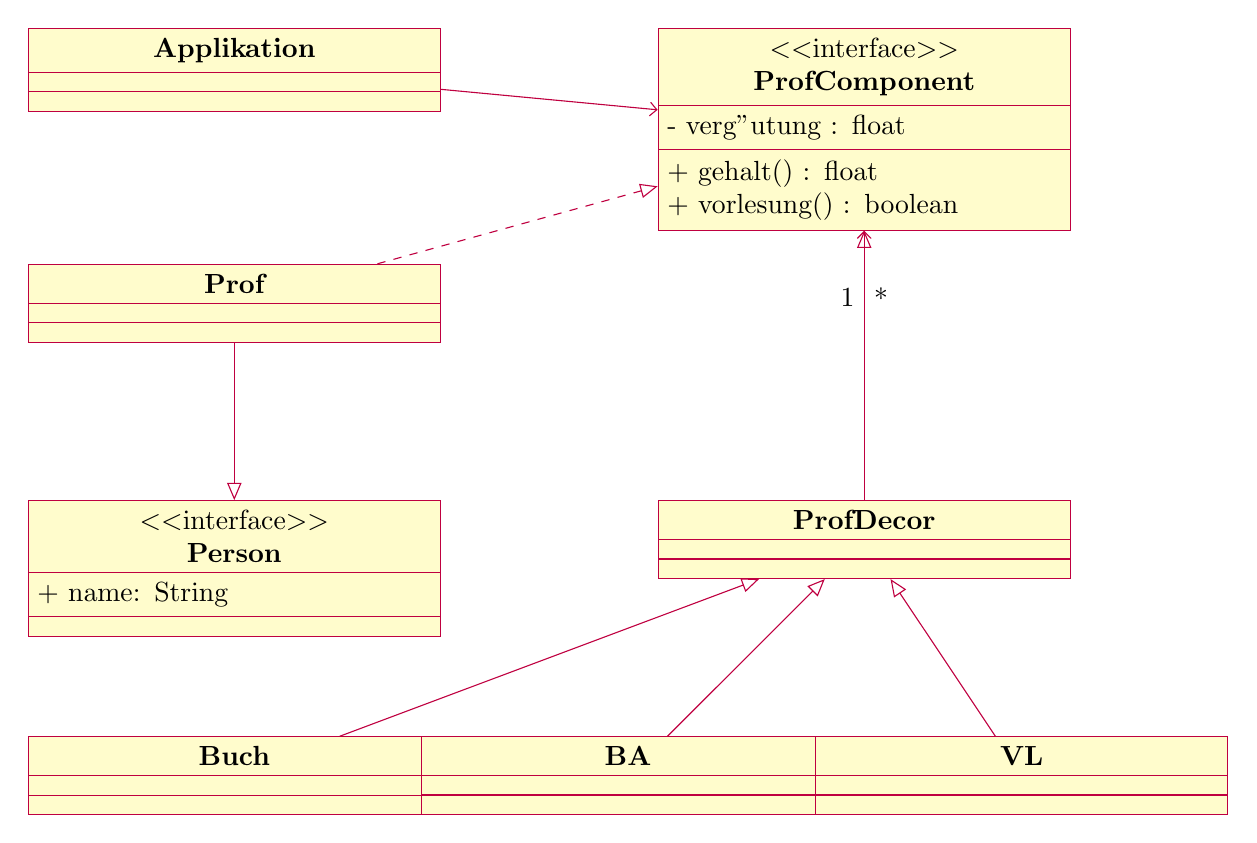
\begin{tikzpicture}

    \begin{class}{Applikation}{0,0}
    \end{class}

    \begin{interface}{ProfComponent}{8,0} 
        \attribute{- verg"utung : float}
        \operation{+ gehalt() : float}
        \operation{+ vorlesung() : boolean}
    \end{interface}
    
    \begin{interface}{Person}{0,-6}
        \attribute{+ name: String}
    \end{interface}
    
    \begin{class}{Prof}{0,-3} 
        \inherit{Person} 
        \implement{ProfComponent}
    \end{class}

    \begin{class}{ProfDecor}{8,-6} 
        \implement{ProfComponent}
    \end{class}
    
    \begin{class}{Buch}{0,-9} 
        \inherit{ProfDecor}
    \end{class}
    
    \begin{class}{BA}{5,-9} 
        \inherit{ProfDecor}
    \end{class}
    
    \begin{class}{VL}{10,-9} 
        \inherit{ProfDecor}
    \end{class}
    

    \unidirectionalAssociation{Applikation}{}{}{ProfComponent}
    \unidirectionalAssociation{ProfDecor}{1}{*}{ProfComponent}

\end{tikzpicture}

\section\

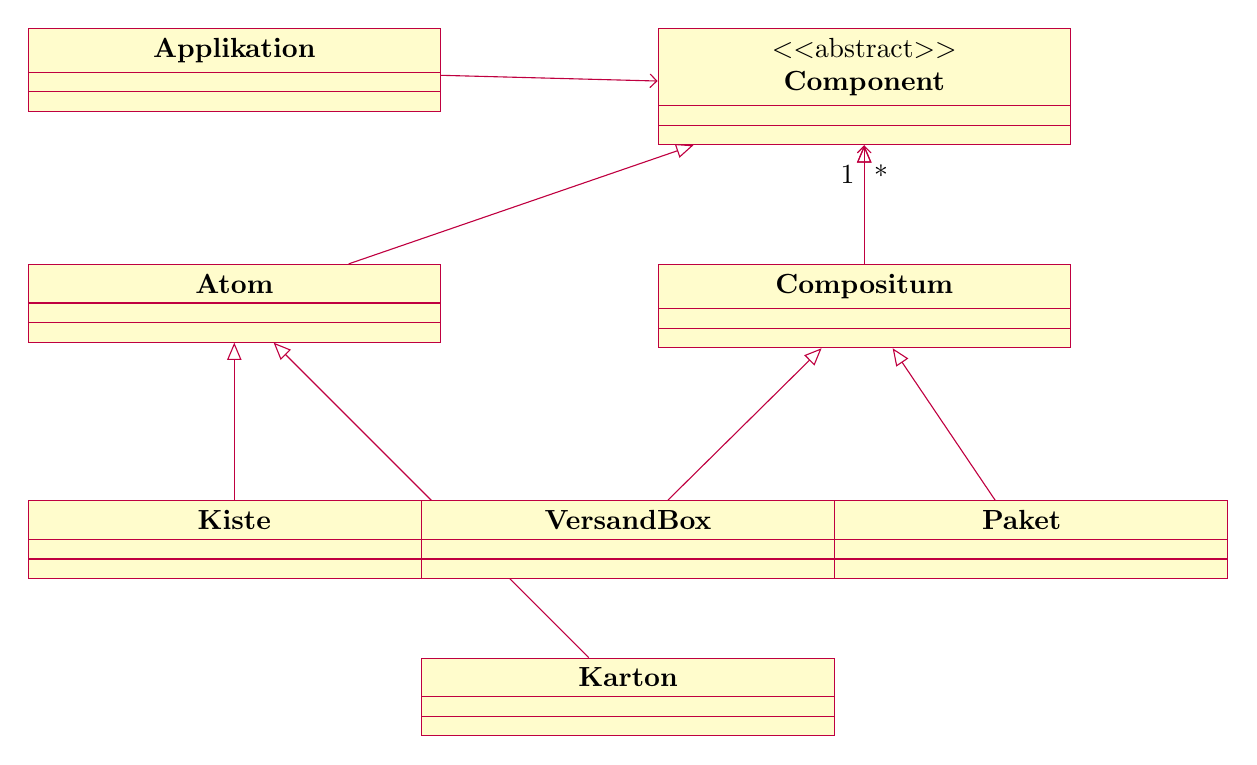
\begin{tikzpicture}

    \begin{class}{Applikation}{0,0}
    \end{class}

    \begin{abstractclass}{Component}{8,0} 
    \end{abstractclass}
    
    \begin{class}{Atom}{0,-3} 
        \inherit{Component} 
    \end{class}

    \begin{class}{Kiste}{0,-6} 
        \inherit{Atom}
    \end{class}

    \begin{class}{Karton}{5,-8} 
        \inherit{Atom}
    \end{class}

    \begin{class}{Compositum}{8,-3} 
        \inherit{Component}
    \end{class}

    \begin{class}{Paket}{10,-6} 
        \inherit{Compositum}
    \end{class}
    
    \begin{class}{VersandBox}{5,-6} 
        \inherit{Compositum}
    \end{class}

    \begin{class}{Compositum}{8,-3} 
        \inherit{Component}
    \end{class}

    \unidirectionalAssociation{Applikation}{}{}{Component}
    \unidirectionalAssociation{Compositum}{1}{*}{Component}

\end{tikzpicture}



%\begin{tikzpicture}
%  \centering
%  \begin{sequencediagram}
%
%    \newthread{A}{Client}{}
%    \newinst[1]{B}{Server}{}
%
%    \begin{call}{A}{Call()}{B}{}
%    \end{call}
%  \end{sequencediagram}
%\end{tikzpicture}
\end{document}
